\hypertarget{introduction}{%
\section{Introduction}\label{introduction}}

Machine-learning models inform credit, hiring, insurance, criminal-justice and clinical decisions, and regulators increasingly require them to be explainable and non-discriminatory \cite{aiact}. Fairness-aware learning formalises group criteria such as demographic parity and enforces them by pre-processing, constrained training or post-processing \cite{zafar,mehrabi,pessach,agarwal,zhang}. Interpretable fuzzy modelling builds rule bases whose antecedents are linguistic terms, so that a prediction can be traced to a few IF--THEN statements \cite{alonso,gacto2011,casillas,mendel}, in line with the argument that high-stakes decisions should rest on interpretable models \cite{rudin}. Combining the two raises two questions that neither line of work answers on its own.

\textbf{Who is in the protected group?} Group criteria assume a crisp partition, for example age ≤ 25 \cite{lequy}. The threshold is a convention, and the measured gap of a fixed classifier can change abruptly when it moves. Continuous attributes have been handled with dependence measures such as covariance \cite{zafar} or the Hirschfeld--Gebelein--Rényi (HGR) correlation \cite{mary}, but these penalise dependence on the attribute as a whole, not a disparity against a named group. A fuzzy protected group keeps the semantics of a group comparison and states the group as a linguistic term with an explicit membership function that a regulator can inspect and change.

\textbf{Does treating similar individuals alike remove group disparity?} A common response to proxy discrimination is to require parity \emph{within} strata of legitimate factors, i.e.~conditional statistical parity \cite{kamiran2013,corbett}. In a rule-based model the rules are natural strata, and it is tempting to require that individuals who match the same rule be treated alike. It has long been known that models can reconstruct a protected attribute from correlated features \cite{pedreschi,lipton} and that constraints on coarse groups can be satisfied while finer subgroups are treated unequally \cite{kearns}. What is missing is a statement of \emph{when} a within-stratum constraint fails if the strata are learned by the model itself, and a measurement device that shows the failure.

We argue that a Takagi--Sugeno--Kang (TSK) rule base \cite{tsk} is such a device. The contributions are:

\begin{enumerate}
\def\labelenumi{\arabic{enumi}.}
\tightlist
\item
  \textbf{Fuzzy demographic parity (FDP).} Parity with respect to a protected group given by a membership function. FDP reduces to demographic parity for crisp groups and has a covariance form (Propositions 1--2). Its plug-in estimator coincides with the probability-weighted estimator used for unobserved protected classes \cite{chen2019,kallus2022}; what is new is its use as an explicit linguistic group specification, as a training objective and in the decomposition below.
\item
  \textbf{Rule-level decomposition.} For any convex mixture of component scores, and in particular for a TSK rule base, the parity gap splits into routing and within-rule terms (Theorem 1), with per-rule shares that do not depend on a common shift of the rule outputs.
\item
  \textbf{Disparity displacement.} A sufficient condition (Theorem 2, Corollary 3) shows that a rule-local penalty cannot move the group gap far from the Bayes gap when a rule base without within-rule disparity is nearly Bayes-optimal, including for regularised and approximately trained models; with a single rule, the rule-local and the group penalty coincide (Corollary 2).
\item
  \textbf{An empirical study} on eight public datasets, with the fuzzy group tested on three of them, and a synthetic benchmark with known Bayes scores, with dataset-level statistics, ten baselines including a fair decision tree and fair rule lists, continuous-attribute penalties, a mixture-of-experts control and a rule-level audit of Adult.
\end{enumerate}

The fairness-aware TSK classifier, called FairTSK below, serves as the measurement device; it is not proposed as a more accurate classifier, and its trade-off matches that of a neural network trained with the same penalty (Section 6.1). The contribution is the definition, the decomposition and the characterisation of a failure mode of local fairness constraints, together with their empirical test; their scope and limits are discussed in Section 7.

Section 2 reviews related work, Section 3 develops FDP, Section 4 the model, the decomposition and the displacement result, Section 5 the experimental protocol and Section 6 the results; Section 7 discusses limitations and Section 8 concludes. Additional results, proofs of auxiliary statements and all tables not needed for the argument are in Online Resource 1 (Sections S1--S8, Tables S1--S25, Figs. S1--S3).

\hypertarget{related-work}{%
\section{Related work}\label{related-work}}

\textbf{Fairness-aware classification.} Group criteria compare decision or error rates across groups \cite{mehrabi,pessach}. Pre-processing reweights or transforms the data \cite{kamiran}; in-processing changes the objective, through covariance constraints \cite{zafar}, reductions to cost-sensitive learning \cite{agarwal}, adversaries that predict the protected attribute \cite{zhang} or HGR penalties for continuous attributes \cite{mary}; post-processing adjusts group-specific thresholds \cite{hardt}. Interpretable-by-design methods impose parity on rule lists \cite{aivodji} and decision trees \cite{barata}, and FairMOE combines interpretable and black-box experts \cite{fairmoe}. Fair representation learning maps inputs to an intermediate representation from which group membership is hard to recover \cite{zemel}; the normalised firing of a rule base is such a learned representation, and Theorem 2 concerns what happens when it is \emph{not} constrained. None of these methods attributes a parity gap exactly to the components of the model.

\textbf{Proxies, strata and subgroups.} Redundant encodings let a model discriminate without the protected attribute \cite{pedreschi}. Lipton et al.~\cite{lipton} showed that parity enforced without access to the protected attribute at prediction time is achieved through proxies of it and can induce discrimination within groups; Kearns et al.~\cite{kearns} showed that parity on coarse groups can hide disparity on subgroups (fairness gerrymandering). Conditional statistical parity requires parity within strata of legitimate factors \cite{kamiran2013,corbett}. Individual fairness \cite{dwork} bounds group parity by how far apart the groups' distributions are. Our displacement result is a precise instance of these concerns for a particular local constraint: parity within \emph{learned}, soft strata, the rules of a mixture model. What the result adds is the condition under which it must occur, its exact measurement and its test where the Bayes score is known.

\textbf{Attributing disparities.} Decomposing a difference of group means into composition and treatment effects is standard in economics (Oaxaca--Blinder \cite{oaxaca,blinder}) and has been revisited for causal disparity analysis \cite{opacic}; Theorem 1 is of this algebraic type. That an aggregate gap and the gaps within strata can differ, even in sign, is the composition effect behind Simpson's paradox, classically illustrated by graduate admissions \cite{bickel}. Post-hoc methods explain individual predictions in terms of features \cite{lime,shap,guidotti}, and Shapley-value methods attribute a model's parity gap to input features \cite{begley}. These answer which \emph{features} carry a gap; Theorem 1 answers which \emph{components of the model} carry it and whether it arises between or within them, which is what a within-component constraint changes.

\textbf{Fuzzy rule-based classifiers and fairness.} ANFIS \cite{anfis} uses grid partitions whose size grows exponentially with \(d\); prototype-based TSK models trained by mini-batch gradient descent scale linearly \cite{mbgd,htsk,zhou,talpur}. Interpretability of rule bases has been studied through complexity and semantic indices \cite{gacto2011,guillaume,gacto2010,alonso}. Fairness objectives have entered fuzzy rule-based classification only recently. Konishi et al.~\cite{konishi} evolve fuzzy rule-based classifiers with multi-objective fuzzy genetics-based machine learning that optimises accuracy and fairness jointly, and analyse the rules of the resulting models; Krasanakis and Papadopoulos \cite{krasanakis} evaluate fairness \emph{statements} in Basic fuzzy logic with crisp groups. The present paper differs from both in defining the protected group itself by a membership function and in decomposing the parity gap of a trained rule base into routing and within-rule parts. The author's earlier conference paper \cite{imam} argued qualitatively for combining fuzzy logic and deep learning for explainability and contains neither the fairness formulation nor the results of this paper.

\hypertarget{fairness-with-respect-to-fuzzy-protected-groups}{%
\section{Fairness with respect to fuzzy protected groups}\label{fairness-with-respect-to-fuzzy-protected-groups}}

Let \((X,Z,Y)\) be drawn from a distribution \(P\), where \(X \in \mathbb{R}^{d}\) are the model inputs, \(Z\) is a sensitive variable (numeric, such as age, or categorical, such as sex) that is not an input, and \(Y \in \{0,1\}\) is the label, with \(Y = 1\) the favourable outcome. The definitions apply to any function \(h\) of \(X\) with values in \([0,1]\): to scores \(\hat y\) and to decisions \(\mathbf{1}[\hat{y} \geq 0.5]\) alike. All statements hold verbatim for the empirical distribution of a sample.

\textbf{Definition 1 (Fuzzy protected group and fuzzy demographic parity).} A fuzzy protected group \(G\) is a fuzzy set on the range of \(Z\) with membership function \(\mu_G\); write \(\mu := \mu_G(Z)\), \(\pi := \mathbb{E}[\mu] \in (0,1)\). The group expectations and the parity gap are \[\mathbb{E}_{G}[h] := \frac{\mathbb{E}[\mu\, h(X)]}{\pi},\qquad \mathbb{E}_{\neg G}[h] := \frac{\mathbb{E}[(1 - \mu)\, h(X)]}{1 - \pi},\qquad \Delta_{G}(h) := \mathbb{E}_{G}[h] - \mathbb{E}_{\neg G}[h], \tag{1}\] and \(\mathrm{FDP}_{G}(h) := |\Delta_{G}(h)|\). We call \(\Delta_G(\hat y)\) the \emph{score-level} and \(\Delta_G(\mathbf{1}[\hat{y} \geq 0.5])\) the \emph{decision-level} gap; all tables report decision-level FDP.

\(\mathbb{E}_G\) is the expectation under \(P\) weighted by \(\mu\), i.e.~Zadeh's probability of a fuzzy event \cite{zadeh68} normalised to a conditional expectation: a person with membership 0.4 contributes with weight 0.4 to the group mean and 0.6 to the complement mean. Intersectional groups are formed with a t-norm, \(\mu_{G_1 \cap G_2} = T(\mu_{G_1},\mu_{G_2})\), which recovers the usual subgroup for crisp memberships.

\textbf{Proposition 1 (Basic properties).} For \(h\) with values in \([0,1]\): (i) if \(\mu \in \{0,1\}\) almost surely, \(\mathrm{FDP}_{G}(h)\) is the classical demographic-parity difference of \(h\); (ii) \(0 \leq \mathrm{FDP}_{G}(h) \leq 1\); (iii) \(\Delta_{\neg G} = -\Delta_{G}\), so FDP does not depend on which of the two groups is called protected.

\emph{Proof.} (i) For crisp \(\mu\), \(\mathbb{E}[\mu h]/\pi = \mathbb{E}[h \mid \mu = 1]\), and likewise for the complement. (ii) Both terms of (1) are averages of values in \([0,1]\). (iii) Exchange \(\mu\) and \(1 - \mu\). \(\square\)

\textbf{Proposition 2 (Covariance form).} For integrable \(h\), \(\Delta_{G}(h) = \mathrm{Cov}(\mu,h)/(\pi(1 - \pi))\); hence \(\mathrm{FDP}_{G}(h) = 0\) if and only if \(\mu\) and \(h\) are uncorrelated.

\emph{Proof.} \(\mathbb{E}[\mu h]/\pi - (\mathbb{E}[h] - \mathbb{E}[\mu h])/(1 - \pi) = (\mathbb{E}[\mu h] - \pi\,\mathbb{E}[h])/(\pi(1 - \pi))\). \(\square\)

\emph{Remark 1 (What is and is not new).} Three readings relate FDP to existing notions. (a) A penalty on \(\Delta_G^2\) is a covariance penalty, as in Zafar et al.~\cite{zafar}; what differs from a penalty on \(\mathrm{Cov}(Z,\hat y)\) is the variable whose dependence is removed: the membership of a named group, not the raw attribute. (b) If \(\tilde G\) is a crisp label drawn with probability \(\mu(Z)\) independently of \((X,Y)\) given \(Z\), then \(\Delta_G(h)\) is the classical parity gap of \(\tilde G\). (c) The plug-in estimate of (1) is the probability-weighted estimator proposed for disparities when the protected class is unobserved \cite{chen2019,kallus2022}. The estimands differ: there the weights are probabilities of an unknown crisp class, here the fuzzy group is the object of interest by definition. The contribution of FDP is therefore not a new estimator but the explicit, inspectable specification of the group and its use in training and in the decomposition of Section 4.

\textbf{The group \emph{young}.} For age we use \(\mu_{\text{young}}(a) = \min\{1,\max\{0,(35 - a)/10\}\}\), which equals 1 up to 25 and 0 from 35. The core reproduces the crisp convention age ≤ 25 \cite{lequy}; the support up to 35 is a normative choice of the analyst, to be agreed like a crisp threshold, by reference to a legal definition, a policy target or expert elicitation, with the support stating explicitly how far protection extends. Section S2 of Online Resource 1 proves that \(\Delta_G\) is Lipschitz in \(\mu\) (Proposition S1), but the constant is conservative (about 5.9 per year of threshold shift on German), so the practical evidence is empirical: the measured gap depends strongly on the location of the group and little on the shape of the transition (Table S2; Table S3; Table S4).

\hypertarget{a-fairness-aware-tsk-classifier-and-its-disparity-decomposition}{%
\section{A fairness-aware TSK classifier and its disparity decomposition}\label{a-fairness-aware-tsk-classifier-and-its-disparity-decomposition}}

\hypertarget{model}{%
\subsection{Model}\label{model}}

A TSK rule base \cite{tsk} has \(L\) rules ``IF \(x_1\) is \(A_{l1}\) AND \ldots{} AND \(x_d\) is \(A_{ld}\) THEN \(y = g_l(x)\)''. The firing strengths are normalised to a soft partition \(\bar w_l(x)\) of the input space and the output is \(\sum_l \bar w_l(x)\, g_l(x)\). FairTSK uses \(L\) rules on the standardised inputs with Gaussian memberships of centres \(c_{lj}\) and widths \(s_{lj}\), raised to powers \(\gamma_{lj} \in (0,1)\): \[\begin{gathered}\log w_{l}(x) = \frac{1}{d}\sum_{j = 1}^{d}\gamma_{lj}\left(-\frac{(x_{j} - c_{lj})^{2}}{2s_{lj}^{2}}\right),\qquad \bar{w}_{l}(x) = \frac{w_l(x)^{1/\tau}}{\sum_{k = 1}^{L}w_k(x)^{1/\tau}},\\ \hat{y}(x) = \sum_{l = 1}^{L}\bar{w}_{l}(x)\,\mathrm{sigmoid}(a_{l}^{\top}x + b_{l}).\end{gathered} \tag{2}\] The factor \(1/d\) is the HTSK device \cite{htsk} that prevents softmax saturation in high dimension; the temperature is \(\tau = 1\). The zero-order variant FairTSK-0 fixes \(g_l \equiv \mathrm{sigmoid}(b_l)\), so that each rule reads ``IF (antecedents) THEN \(P(Y = 1) = g_l\)''. Feature \(j\) enters rule \(l\) only through the effective precision \(P_{lj} = \gamma_{lj}/(2s_{lj}^2)\), so \(\gamma_{lj}\) alone is not identifiable; we measure antecedent relevance by the scale-invariant \(\varrho_{lj} := P_{lj}\mathrm{Var}(x_j)\). The cost of a training epoch is \(O(nLd)\), linear in the numbers of samples, rules and features (Section S8 of Online Resource 1). The architecture combines known components; we do not claim it as a contribution.

FairTSK minimises \[\mathcal{L} = \mathrm{BCE}(y,\hat{y}) + \lambda_{f}\,\Omega_{\text{fair}} + \lambda_{b}\,\mathrm{KL}(\bar{u}\,\|\,\mathcal{U}_{L}) + \frac{\lambda_{a}}{Ld}\sum_{l,j}|a_{lj}| + \frac{\lambda_{\gamma}}{Ld}\sum_{l,j}\gamma_{lj}, \tag{3}\] where \(\bar{u}\) is the mean rule usage in a mini-batch; the load-balancing term prevents rule collapse, as in mixtures of experts \cite{shazeer}, and the last two terms regularise the consequents and the gates. The total fairness penalty is \(\Omega_{\text{fair}} = \hat{\Delta}_{G}(\hat y)^{2}\), the squared mini-batch estimate of Proposition 2.

\hypertarget{rule-level-decomposition}{%
\subsection{Rule-level decomposition}\label{rule-level-decomposition}}

For rule \(l\) and \(H \in \{G,\neg G\}\) let \(m_{l}^{H} := \mathbb{E}_{H}[\bar{w}_{l}]\) (coverage) and \(r_{l}^{H} := \mathbb{E}_{H}[\bar{w}_{l}\, g_{l}]/m_{l}^{H}\) (within-rule rate), with midpoints \(\bar{m}_{l}\) and \(\bar{r}_{l}\).

\textbf{Theorem 1 (Rule-level decomposition).} If \(\hat y = \sum_l \bar w_l g_l\) with \(\bar w_l > 0\), \(\sum_l \bar w_l = 1\) and \(g_l \in [0,1]\), then for any fuzzy group \(G\) \[\Delta_{G}(\hat{y}) = \mathcal{R} + \mathcal{W},\qquad \mathcal{R} := \sum_{l = 1}^{L}(m_{l}^{G} - m_{l}^{\neg G})\,\bar{r}_{l},\qquad \mathcal{W} := \sum_{l = 1}^{L}\bar{m}_{l}\,(r_{l}^{G} - r_{l}^{\neg G}). \tag{4}\]

\emph{Proof.} By linearity and \(\sum_l \bar w_l = 1\), \(\mathbb{E}_{H}[\hat{y}] = \sum_{l}m_{l}^{H}r_{l}^{H}\); apply \(ab - a'b' = (a - a')(b + b')/2 + (a + a')(b - b')/2\) termwise. \(\square\)

\(\mathcal R\), the \emph{routing} disparity, is non-zero when the groups are covered by different rules that carry different outcomes; \(\mathcal W\), the \emph{within-rule} disparity, when individuals who fire the same rule receive different scores by group. \textbf{Corollary 1.} If every \(g_l\) is constant (FairTSK-0), then \(\mathcal W = 0\): every disparity is routing.

Because \(\sum_l (m_l^G - m_l^{\neg G}) = 0\), \(\mathcal R = \sum_l (m_l^G - m_l^{\neg G})(\bar r_l - c)\) for any constant \(c\). The midpoint weights in (4) avoid the index-number choice of Oaxaca--Blinder analysis, in which the coverage or the rates of one group serve as reference; Section 6.3 reports the split under both alternatives. We define the \emph{share} of rule \(l\) as \((m_l^G - m_l^{\neg G})(\bar r_l - c) + \bar m_l (r_l^G - r_l^{\neg G})\) with \(c\) the mean score; the shares sum to the gap and do not change when a constant is added to all rule outputs. A rule contributes to the gap if one group is over-represented in it and its outcome differs from the average.

Theorem 1 is an Oaxaca--Blinder-type identity \cite{oaxaca,blinder} and holds for any convex mixture, including mixtures of experts \cite{jacobs,shazeer} and the leaves of a decision tree. Two qualifications matter for its use. First, the split between \(\mathcal R\) and \(\mathcal W\) depends on how the predictor is parametrised: with one rule all disparity is within-rule, with many narrow rules most of it is routing. It describes the computation of the fitted model, not the causes of the disparity in the data. Second, it decomposes the score-level gap, the difference of mean predicted probabilities; thresholding is not linear, and no exact identity holds for decisions. The two gaps are different quantities rather than one being a part of the other: on COMPAS without a penalty the score-level gap is −0.117 and the decision-level gap 0.227, because thresholding at 0.5 amplifies differences of scores near the threshold. Across the 1,050 trained TSK models of the main comparison, the absolute score-level gap and the decision-level FDP correlate at 0.82 (per dataset 0.70--0.99, except Diabetes, where both are essentially zero; Table S16).

\hypertarget{when-must-a-rule-local-penalty-fail}{%
\subsection{When must a rule-local penalty fail?}\label{when-must-a-rule-local-penalty-fail}}

Conditional statistical parity requires parity within strata of legitimate factors \cite{kamiran2013,corbett}. In a rule base, the rules are learned soft strata, and requiring that ``individuals who match the same rule be treated alike'' gives the \emph{rule-local} penalty \[\Omega(\hat y) := \sum_{l}\bar{m}_{l}\,(r_{l}^{G} - r_{l}^{\neg G})^{2}, \tag{5}\] which penalises \(\mathcal W\) (Lemma 1) and leaves routing free. We call the resulting model FairTSK-rule. The question is whether such a constraint reduces the group gap when the strata are chosen by the optimiser. Let \(\eta(x) = P(Y = 1 \mid X = x)\), \(\mathcal{L}_{\log}(f)\) the population log-loss and \(\varepsilon(f) := \mathcal{L}_{\log}(f) - \mathcal{L}_{\log}(\eta) = \mathbb{E}\,\mathrm{KL}(\mathrm{Ber}(\eta)\,\|\,\mathrm{Ber}(f))\) the excess risk.

\textbf{Lemma 1.} For any convex mixture: (a) \(|\mathcal{W}| \leq \sqrt{\Omega}\); (b) if every \(g_l\) is constant, \(\Omega = 0\); (c) if \(L = 1\), then \(\mathcal{R} = 0\) and \(\Omega = \mathcal W^2 = \Delta_{G}^{2}\).

\emph{Proof.} (a) Cauchy--Schwarz with weights \(\bar m_l\) summing to one. (b) Corollary 1. (c) With one rule \(\bar w_1 \equiv 1\), so \(m_1^G = m_1^{\neg G} = 1\). \(\square\)

\textbf{Proposition 3 (Excess risk controls the gap).} For every score \(f\), \[|\Delta_{G}(f) - \Delta_{G}(\eta)| \leq \kappa_{\mu}\sqrt{\frac{\varepsilon(f)}{2\pi(1 - \pi)}},\qquad \kappa_{\mu} := \sqrt{\frac{\mathrm{Var}(\mu)}{\pi(1 - \pi)}} \in [0,1], \tag{6}\] with \(\kappa_{\mu} = 1\) if and only if \(\mu\) is crisp.

\emph{Proof.} By Proposition 2, \(\Delta_{G}(f) - \Delta_{G}(\eta) = \mathrm{Cov}(\mu,f - \eta)/(\pi(1 - \pi))\). Cauchy--Schwarz gives \(|\mathrm{Cov}(\mu,f - \eta)| \leq \sqrt{\mathrm{Var}(\mu)\,\mathbb{E}[(f - \eta)^{2}]}\), and Pinsker's inequality \cite{cover} gives \(\mathbb{E}[(f - \eta)^{2}] \leq \varepsilon(f)/2\). Finally \(\mathrm{Var}(\mu) \leq \pi - \pi^{2}\) for \(\mu \in [0,1]\), with equality if and only if \(\mu^2 = \mu\). \(\square\)

\textbf{Theorem 2 (Disparity displacement).} Let \(\mathcal{M}\) be a class of \(L\)-component convex mixtures, \(f_{\lambda}\) a minimiser of \(\mathcal{L}_{\log}(f) + \lambda\,\Omega(f)\) over \(\mathcal{M}\) (assumed to exist; otherwise Corollary 3 applies to any \(f\) whose objective is within \(\delta > 0\) of the infimum), and \(\varepsilon_{\Omega} := \inf\{\varepsilon(f): f \in \mathcal{M},\ \Omega(f) = 0\}\). Then for every \(\lambda \geq 0\): (i) \(\varepsilon(f_{\lambda}) \leq \varepsilon_{\Omega}\); (ii) \(|\Delta_{G}(f_{\lambda}) - \Delta_{G}(\eta)| \leq \kappa_{\mu}\sqrt{\varepsilon_{\Omega}/(2\pi(1 - \pi))}\); (iii) for \(\lambda > 0\), \(|\mathcal{W}(f_{\lambda})| \leq \sqrt{\varepsilon_{\Omega}/\lambda}\). If \(\mathcal{M}\) contains its zero-order members, \(\varepsilon_{\Omega}\) is at most the excess risk \(\varepsilon_{0}\) of the best zero-order rule base.

\emph{Proof.} Let \(f' \in \mathcal{M}\) with \(\Omega(f') = 0\). (i) \(\mathcal{L}_{\log}(f_{\lambda}) \leq \mathcal{L}_{\log}(f_{\lambda}) + \lambda\Omega(f_\lambda) \leq \mathcal{L}_{\log}(f')\); subtract \(\mathcal{L}_{\log}(\eta)\) and take the infimum. (ii) Proposition 3 and (i). (iii) \(\lambda\Omega(f_{\lambda}) \leq \mathcal{L}_{\log}(f') - \mathcal{L}_{\log}(f_\lambda) \leq \varepsilon(f')\); take the infimum and apply Lemma 1(a). The last claim follows from Lemma 1(b). \(\square\)

\textbf{Corollary 2 (One rule).} If \(L = 1\), the rule-local penalty equals \(\lambda\Delta_G^2\), the group penalty (Lemma 1(c)); if \(\mathcal M\) contains a constant score \(f_c\), then \(\lambda\Delta_{G}(f_\lambda)^2 \le \mathcal{L}_{\log}(f_c)\), so \(\Delta_{G}(f_\lambda) \to 0\) as \(\lambda \to \infty\).

\textbf{Corollary 3 (Regularised objectives and approximate minimisers).} Let \(\Psi \geq 0\) be any additional regulariser (for FairTSK, the last three terms of (3)), \(\tilde J_\lambda = \mathcal{L}_{\log} + \lambda\Omega + \Psi\), and let \(\hat f\) satisfy \(\tilde J_\lambda(\hat f) \leq \tilde J_\lambda(f') + \delta\) for some \(f'\) with \(\Omega(f') = 0\). Then (i)--(iii) of Theorem 2 hold for \(\hat f\) with \(\varepsilon_\Omega\) replaced by \(\tilde\varepsilon := \varepsilon(f') + \Psi(f') + \delta\).

\emph{Proof.} \(\mathcal{L}_{\log}(\hat f) \leq \tilde J_\lambda(\hat f) \leq \mathcal{L}_{\log}(f') + \Psi(f') + \delta\); subtract \(\mathcal{L}_{\log}(\eta)\) and apply Proposition 3. Similarly \(\lambda\Omega(\hat f) \leq \tilde J_\lambda(\hat f) - \mathcal{L}_{\log}(\hat f) \leq \tilde\varepsilon\) because \(\mathcal{L}_{\log}(\hat f) \geq \mathcal{L}_{\log}(\eta)\). \(\square\)

\textbf{Interpretation.} A rule-local penalty cannot remove a group gap when (i) the inputs carry information about the group that the Bayes score uses, so that \(\Delta_{G}(\eta) \neq 0\), and (ii) the antecedents can partition the input space finely enough that some rule base without within-rule disparity is nearly Bayes-optimal. The penalty is then free: \(\mathcal W\) vanishes at rate \(\lambda^{-1/2}\) while the gap stays near the Bayes gap and is carried by routing. With a single rule or fixed antecedents, routing capacity is small and the penalty acts on the gap. Part (ii) holds for every \(\lambda\), including \(\lambda = 0\); its content is that the penalty does not pull the solution away from the Bayes score. The constant from Cauchy--Schwarz and Pinsker is not tight, and \(\varepsilon_\Omega\) requires \(\eta\), so the theorem can be verified on synthetic data (Section 6.4) but not on real data. There, a zero-order rule base that is nearly as accurate as the first-order one is a necessary sign that \(\varepsilon_0\) is small, not a sufficient one.

\hypertarget{experimental-setup}{%
\section{Experimental setup}\label{experimental-setup}}

\textbf{Datasets.} We use eight public tabular datasets that are standard in fairness research \cite{lequy} (Table 1): German Credit \cite{german}, Student Performance \cite{student}, COMPAS \cite{compas}, Default of Credit Card Clients \cite{default}, Bank Marketing \cite{bank}, Adult \cite{adult}, Diabetes 130-US Hospitals \cite{diabetes} and Census-Income (KDD) \cite{censuskdd}. Three leakage problems were removed: the call duration in Bank, which is known only after the outcome \cite{bank}; the period grades G1 and G2 in Student; and patient overlap in Diabetes, which is split by patient. The COMPAS risk score is not an input. Census-KDD uses a stratified subsample of 60,000 training instances per split. The protected attribute is never an input. For German and Bank the group is the fuzzy set \emph{young}, and the crisp baselines use its core (age ≤ 25); elsewhere the group is crisp, so that FDP is classical demographic parity (Proposition 1). We follow the benchmark convention \cite{lequy} for the protected attribute; by Proposition 1(iii) FDP does not depend on which group is called protected, which matters for Default, where women have the higher favourable rate. Diabetes is a \emph{control} with almost equal rates. A ninth setting tests the fuzzy group on a large dataset: Adult with \emph{young} as the protected group (age and sex are not inputs; favourable rate 0.02 for age ≤ 25 and 0.07 membership-weighted, against 0.30 for age \textgreater{} 25), run with the full protocol on 10 splits and reported separately (Sections 6.1 and 6.3).

\begin{longtable}[]{@{}
  >{\raggedright\arraybackslash}p{(\columnwidth - 12\tabcolsep) * \real{0.1429}}
  >{\raggedright\arraybackslash}p{(\columnwidth - 12\tabcolsep) * \real{0.1429}}
  >{\raggedright\arraybackslash}p{(\columnwidth - 12\tabcolsep) * \real{0.1429}}
  >{\raggedright\arraybackslash}p{(\columnwidth - 12\tabcolsep) * \real{0.1429}}
  >{\raggedright\arraybackslash}p{(\columnwidth - 12\tabcolsep) * \real{0.1429}}
  >{\raggedright\arraybackslash}p{(\columnwidth - 12\tabcolsep) * \real{0.1429}}
  >{\raggedright\arraybackslash}p{(\columnwidth - 12\tabcolsep) * \real{0.1429}}@{}}
\caption{Datasets after preprocessing: \(n\) instances, \(d\) encoded features, and the favourable-outcome rate overall, in the group \(G\) and in its complement (membership-weighted for fuzzy groups).}\tabularnewline
\toprule\noalign{}
\begin{minipage}[b]{\linewidth}\raggedright
\textbf{Dataset}
\end{minipage} & \begin{minipage}[b]{\linewidth}\raggedright
\(n\)
\end{minipage} & \begin{minipage}[b]{\linewidth}\raggedright
\(d\)
\end{minipage} & \begin{minipage}[b]{\linewidth}\raggedright
\textbf{Group} \(G\)
\end{minipage} & \begin{minipage}[b]{\linewidth}\raggedright
\(P(Y = 1)\)
\end{minipage} & \begin{minipage}[b]{\linewidth}\raggedright
\(P(Y = 1 \mid G)\)
\end{minipage} & \begin{minipage}[b]{\linewidth}\raggedright
\(P(Y = 1 \mid \neg G)\)
\end{minipage} \\
\midrule\noalign{}
\endfirsthead
\toprule\noalign{}
\begin{minipage}[b]{\linewidth}\raggedright
\textbf{Dataset}
\end{minipage} & \begin{minipage}[b]{\linewidth}\raggedright
\(n\)
\end{minipage} & \begin{minipage}[b]{\linewidth}\raggedright
\(d\)
\end{minipage} & \begin{minipage}[b]{\linewidth}\raggedright
\textbf{Group} \(G\)
\end{minipage} & \begin{minipage}[b]{\linewidth}\raggedright
\(P(Y = 1)\)
\end{minipage} & \begin{minipage}[b]{\linewidth}\raggedright
\(P(Y = 1 \mid G)\)
\end{minipage} & \begin{minipage}[b]{\linewidth}\raggedright
\(P(Y = 1 \mid \neg G)\)
\end{minipage} \\
\midrule\noalign{}
\endhead
\bottomrule\noalign{}
\endlastfoot
German & 1,000 & 60 & fuzzy \emph{young} & 0.700 & 0.638 & 0.739 \\
Student & 649 & 54 & sex (male) & 0.846 & 0.812 & 0.869 \\
COMPAS & 6,172 & 9 & race (African-American) & 0.545 & 0.477 & 0.617 \\
Default & 30,000 & 31 & sex (female) & 0.779 & 0.792 & 0.758 \\
Bank & 45,211 & 49 & fuzzy \emph{young} & 0.117 & 0.153 & 0.110 \\
Adult & 45,222 & 86 & sex (female) & 0.248 & 0.114 & 0.312 \\
Diabetes & 101,763 & 221 & race (African-American) & 0.888 & 0.888 & 0.889 \\
Census-KDD & 299,285 & 469 & sex (female) & 0.062 & 0.025 & 0.102 \\
\end{longtable}

\textbf{Compared methods.} All methods receive the same inputs, splits and preprocessing.

\begin{itemize}
\tightlist
\item
  Unconstrained references: logistic regression (LR), LightGBM \cite{lightgbm} and a two-layer ReLU network (DNN).
\item
  Reweighing \cite{kamiran} on LightGBM; Exponentiated Gradient \cite{agarwal} with an LR base learner (Fairlearn \cite{fairlearn}); adversarial debiasing \cite{zhang}; Threshold Optimizer \cite{hardt}, which uses the group label at prediction time.
\item
  \textbf{DNN+FDP}, the DNN trained with exactly the FDP penalty of FairTSK. It shares FairTSK's objective but not its architecture, so a difference between the two isolates the rule base.
\item
  Interpretable fairness-aware models: the fair decision tree of Barata et al.~\cite{barata} (package fair-trees 3.1.9) and FairCORELS rule lists \cite{aivodji} (version 1.0) on binarised inputs.
\item
  On German and Bank, where the sensitive variable is numeric: the DNN with a covariance penalty on age, with a kernel-density HGR-type penalty \cite{mary}, and logistic regression with the covariance constraint of Zafar et al.~\cite{zafar} on the crisp group or on age.
\item
  FairTSK (total penalty), FairTSK-0 (zero-order) and FairTSK-rule (rule-local penalty (5)), with \(L = 16\); the \(\lambda_f = 0\) member of each family is the unconstrained TSK model.
\end{itemize}

Each family is run on a small fixed grid of its trade-off parameter; the grids and all hyperparameters, with their origin (a priori, pilot or validation), are listed in Table S1. No hyperparameter was tuned on test data.

\textbf{Protocol.} Data are split 60/20/20, stratified by label and group, on 10 random splits (5 for Diabetes and Census-KDD). Networks and TSK models are trained with Adam \cite{adam} for at most 100 epochs with early stopping on the validation objective. For each family, split and parity target \(\epsilon = 0.05\), the \emph{operating point} is the configuration with the highest validation accuracy among those with validation FDP ≤ \(\epsilon\) (else the smallest validation FDP). Each family's whole trade-off is summarised by the normalised hypervolume (HV) \cite{zitzler} of its (FDP, accuracy) points with reference point (FDP = 0.2, majority-class accuracy): \[\mathrm{HV} = \frac{1}{(1 - \text{acc}_{\text{ref}})\cdot 0.2}\ \mathrm{area}\Big(\bigcup_i\,[\text{FDP}_i,\,0.2] \times [\text{acc}_{\text{ref}},\,\text{acc}_i]\Big). \tag{7}\] HV favours families with more configurations and, computed from all test points, selects the front on test data. We therefore also report the HV of the \emph{validation-selected front} (configurations non-dominated on validation data, evaluated on test data), and a sensitivity analysis for the reference FDP of 0.1 and 0.3.

\textbf{Statistics.} Random splits share most of their training data, so all cross-dataset inference uses one value per dataset, the mean over its splits (\(N = 8\)): the Friedman test, and Wilcoxon signed-rank tests of FairTSK against each competitor with Holm's correction \cite{demsar,holm}. With \(N = 8\) the smallest two-sided Wilcoxon \(p\)-value is 0.0078, so these tests have little power. For FairTSK versus DNN+FDP we report 90\% confidence intervals of the dataset-level difference; no equivalence margin was fixed in advance, so we do not claim equivalence \cite{schuirmann}. Comparisons over the splits of one dataset use the Nadeau--Bengio corrected resampled \(t\)-test \cite{nadeau}.

\textbf{Synthetic study.} To test Theorem 2 where \(\eta\) is known, \(x = (z_1,z_2,z_3) \sim \mathcal{N}(0,I_3)\) and \(Y \mid x \sim \mathrm{Ber}(\eta(x))\) with a linear logit \(-0.5 + 1.5z_1 + z_2 - z_3\) or a nonlinear logit \(-0.5 + 1.5z_1 + 2\sin(2.5z_2) + 1.5z_2z_3\). A latent age \(a = 40 + 10(\rho z_1 + \sqrt{1 - \rho^2}\,e)\), \(e \sim \mathcal{N}(0,1)\), not an input, defines \(\mu = \mu_{\text{young}}(a)\); \(\rho\) sets how much group information the inputs carry. Routing capacity is varied through \(L \in \{1,2,4,8,16,32\}\) and by freezing the antecedents. Each configuration is trained without penalty, with the rule-local penalty and, for selected configurations, with the total penalty (\(\lambda = 100\)), on 20,000/10,000/50,000 training, validation and test points with 5 seeds: 700 runs over \(\rho \in \{0,0.3,0.6,0.9\}\) (linear) and \(\rho = 0.6\) (nonlinear). \(\varepsilon(f)\) is estimated by Monte Carlo as the mean Bernoulli divergence over the 50,000 test inputs, and \(\varepsilon_\Omega\) is bounded by the excess risk \(\hat\varepsilon_0\) of a zero-order rule base with the same \(L\) and antecedent mode. To check Corollary 3, 80 rule-local runs (\(\rho = 0.6\), \(L \in \{2,4,8,16\}\), trainable antecedents) were repeated under the regularised objective (3) with early stopping and under a \emph{plain} protocol (log-loss and penalty only, 100 epochs, last iterate).

\textbf{Implementation and use of AI tools.} All models are implemented in PyTorch \cite{pytorch}, except LR (scikit-learn), LightGBM and the Fairlearn baselines; runs used one CPU thread with fixed seeds. Code, per-split results and the scripts that regenerate every table and figure are publicly available \cite{software}. Claude (Anthropic), a large language model, was used to assist with literature search, drafting and language editing, writing and debugging the experimental code, and producing tables and figures from the results. All results were computed by the released code; the author reviewed all content, verified the proofs and the results, and takes full responsibility for the article.

\hypertarget{results}{%
\section{Results}\label{results}}

\hypertarget{accuracyfairness-trade-off}{%
\subsection{Accuracy--fairness trade-off}\label{accuracyfairness-trade-off}}

Table 2 reports the HV of each family's test front, Fig. 1 the fronts and Table 3 the dataset-level comparisons; operating points and further metrics are in Table S5 and Table S6.

\begin{longtable}[]{@{}
  >{\raggedright\arraybackslash}p{(\columnwidth - 16\tabcolsep) * \real{0.1111}}
  >{\raggedright\arraybackslash}p{(\columnwidth - 16\tabcolsep) * \real{0.1111}}
  >{\raggedright\arraybackslash}p{(\columnwidth - 16\tabcolsep) * \real{0.1111}}
  >{\raggedright\arraybackslash}p{(\columnwidth - 16\tabcolsep) * \real{0.1111}}
  >{\raggedright\arraybackslash}p{(\columnwidth - 16\tabcolsep) * \real{0.1111}}
  >{\raggedright\arraybackslash}p{(\columnwidth - 16\tabcolsep) * \real{0.1111}}
  >{\raggedright\arraybackslash}p{(\columnwidth - 16\tabcolsep) * \real{0.1111}}
  >{\raggedright\arraybackslash}p{(\columnwidth - 16\tabcolsep) * \real{0.1111}}
  >{\raggedright\arraybackslash}p{(\columnwidth - 16\tabcolsep) * \real{0.1111}}@{}}
\caption{Normalised hypervolume (7) of the test accuracy--FDP front (mean ± s.d. over splits; higher is better). Best per dataset in bold.}\tabularnewline
\toprule\noalign{}
\begin{minipage}[b]{\linewidth}\raggedright
\textbf{Method}
\end{minipage} & \begin{minipage}[b]{\linewidth}\raggedright
\textbf{German}
\end{minipage} & \begin{minipage}[b]{\linewidth}\raggedright
\textbf{Student}
\end{minipage} & \begin{minipage}[b]{\linewidth}\raggedright
\textbf{COMPAS}
\end{minipage} & \begin{minipage}[b]{\linewidth}\raggedright
\textbf{Default}
\end{minipage} & \begin{minipage}[b]{\linewidth}\raggedright
\textbf{Bank}
\end{minipage} & \begin{minipage}[b]{\linewidth}\raggedright
\textbf{Adult}
\end{minipage} & \begin{minipage}[b]{\linewidth}\raggedright
\textbf{Diabetes}
\end{minipage} & \begin{minipage}[b]{\linewidth}\raggedright
\textbf{Census-KDD}
\end{minipage} \\
\midrule\noalign{}
\endfirsthead
\toprule\noalign{}
\begin{minipage}[b]{\linewidth}\raggedright
\textbf{Method}
\end{minipage} & \begin{minipage}[b]{\linewidth}\raggedright
\textbf{German}
\end{minipage} & \begin{minipage}[b]{\linewidth}\raggedright
\textbf{Student}
\end{minipage} & \begin{minipage}[b]{\linewidth}\raggedright
\textbf{COMPAS}
\end{minipage} & \begin{minipage}[b]{\linewidth}\raggedright
\textbf{Default}
\end{minipage} & \begin{minipage}[b]{\linewidth}\raggedright
\textbf{Bank}
\end{minipage} & \begin{minipage}[b]{\linewidth}\raggedright
\textbf{Adult}
\end{minipage} & \begin{minipage}[b]{\linewidth}\raggedright
\textbf{Diabetes}
\end{minipage} & \begin{minipage}[b]{\linewidth}\raggedright
\textbf{Census-KDD}
\end{minipage} \\
\midrule\noalign{}
\endhead
\bottomrule\noalign{}
\endlastfoot
Reweighing & 0.121 ±~0.075 & 0.051 ±~0.060 & 0.012 ±~0.018 & 0.160 ±~0.017 & 0.083 ±~0.014 & 0.195 ±~0.017 & \textbf{0.013 ±~0.022} & 0.202 ±~0.024 \\
Exp. Gradient & 0.113 ±~0.040 & 0.071 ±~0.079 & 0.067 ±~0.024 & 0.131 ±~0.020 & 0.078 ±~0.012 & 0.303 ±~0.025 & 0.010 ±~0.021 & 0.199 ±~0.028 \\
Threshold Opt. & 0.112 ±~0.067 & 0.001 ±~0.001 & \textbf{0.153 ±~0.039} & 0.165 ±~0.019 & 0.088 ±~0.019 & \textbf{0.357 ±~0.022} & \textbf{0.013 ±~0.024} & 0.145 ±~0.026 \\
Adv. debiasing & 0.130 ±~0.041 & \textbf{0.096 ±~0.107} & 0.012 ±~0.023 & 0.161 ±~0.022 & 0.088 ±~0.012 & 0.182 ±~0.061 & 0.012 ±~0.022 & 0.190 ±~0.027 \\
DNN+FDP & 0.174 ±~0.032 & 0.081 ±~0.078 & 0.106 ±~0.020 & 0.173 ±~0.022 & \textbf{0.095 ±~0.009} & 0.354 ±~0.011 & 0.012 ±~0.022 & 0.216 ±~0.030 \\
FairTSK & 0.172 ±~0.037 & 0.080 ±~0.037 & 0.104 ±~0.022 & 0.179 ±~0.022 & \textbf{0.095 ±~0.011} & 0.354 ±~0.009 & 0.012 ±~0.022 & \textbf{0.219 ±~0.028} \\
FairTSK-0 & \textbf{0.176 ±~0.058} & 0.034 ±~0.054 & 0.090 ±~0.020 & \textbf{0.182 ±~0.018} & 0.082 ±~0.009 & 0.351 ±~0.014 & 0.011 ±~0.022 & 0.214 ±~0.027 \\
\end{longtable}

\begin{figure}
\centering
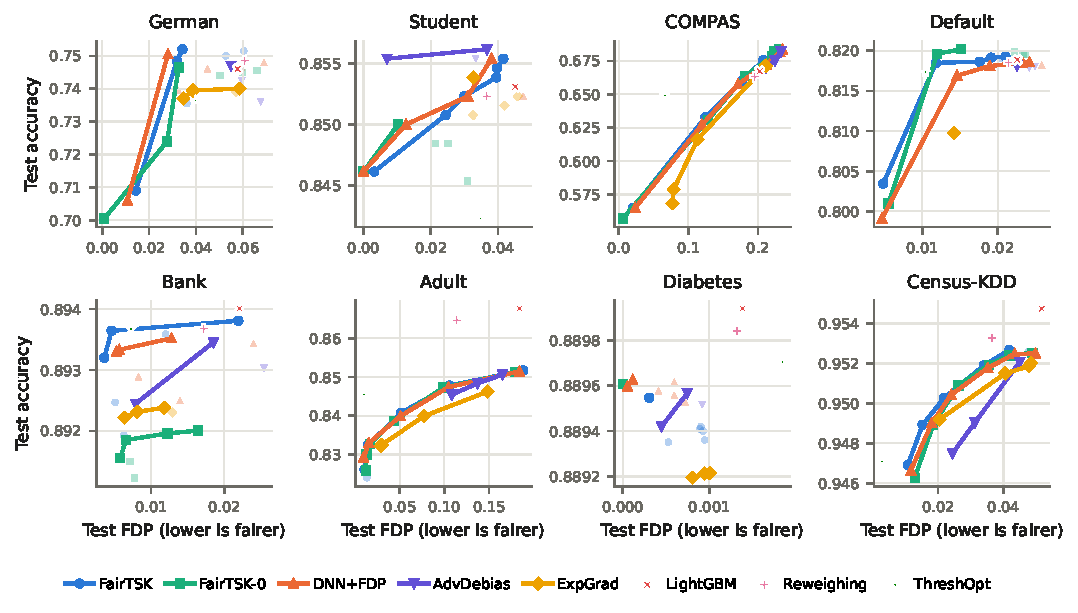
\includegraphics[width=1\textwidth,height=\textheight]{figures/fig_pareto.pdf}
\caption{Test accuracy versus FDP. Large markers joined by lines: non-dominated configurations of each family (means over splits); faint markers: all configurations; single markers: methods without a trade-off parameter. Lower FDP is fairer}
\end{figure}

\begin{longtable}[]{@{}
  >{\raggedright\arraybackslash}p{(\columnwidth - 14\tabcolsep) * \real{0.1250}}
  >{\raggedright\arraybackslash}p{(\columnwidth - 14\tabcolsep) * \real{0.1250}}
  >{\raggedright\arraybackslash}p{(\columnwidth - 14\tabcolsep) * \real{0.1250}}
  >{\raggedright\arraybackslash}p{(\columnwidth - 14\tabcolsep) * \real{0.1250}}
  >{\raggedright\arraybackslash}p{(\columnwidth - 14\tabcolsep) * \real{0.1250}}
  >{\raggedright\arraybackslash}p{(\columnwidth - 14\tabcolsep) * \real{0.1250}}
  >{\raggedright\arraybackslash}p{(\columnwidth - 14\tabcolsep) * \real{0.1250}}
  >{\raggedright\arraybackslash}p{(\columnwidth - 14\tabcolsep) * \real{0.1250}}@{}}
\caption{Dataset-level comparison of FairTSK with each fairness-aware method (\(N = 8\); one value per dataset). Δ = FairTSK minus competitor; wins = datasets with larger test-front HV; \(p_{Holm}\): Wilcoxon signed-rank test, Holm-adjusted within each column group. Confidence intervals are not adjusted for multiplicity.}\tabularnewline
\toprule\noalign{}
\begin{minipage}[b]{\linewidth}\raggedright
\textbf{FairTSK vs.}
\end{minipage} & \begin{minipage}[b]{\linewidth}\raggedright
\textbf{Δ HV, test front {[}90\% CI{]}}
\end{minipage} & \begin{minipage}[b]{\linewidth}\raggedright
\textbf{wins/8}
\end{minipage} & \begin{minipage}[b]{\linewidth}\raggedright
\(p_{Holm}\)
\end{minipage} & \begin{minipage}[b]{\linewidth}\raggedright
\textbf{Δ HV, validation-selected front {[}90\% CI{]}}
\end{minipage} & \begin{minipage}[b]{\linewidth}\raggedright
\(p_{Holm}\)
\end{minipage} & \begin{minipage}[b]{\linewidth}\raggedright
\textbf{Δ acc@0.05 {[}90\% CI{]}}
\end{minipage} & \begin{minipage}[b]{\linewidth}\raggedright
\(p_{Holm}\)
\end{minipage} \\
\midrule\noalign{}
\endfirsthead
\toprule\noalign{}
\begin{minipage}[b]{\linewidth}\raggedright
\textbf{FairTSK vs.}
\end{minipage} & \begin{minipage}[b]{\linewidth}\raggedright
\textbf{Δ HV, test front {[}90\% CI{]}}
\end{minipage} & \begin{minipage}[b]{\linewidth}\raggedright
\textbf{wins/8}
\end{minipage} & \begin{minipage}[b]{\linewidth}\raggedright
\(p_{Holm}\)
\end{minipage} & \begin{minipage}[b]{\linewidth}\raggedright
\textbf{Δ HV, validation-selected front {[}90\% CI{]}}
\end{minipage} & \begin{minipage}[b]{\linewidth}\raggedright
\(p_{Holm}\)
\end{minipage} & \begin{minipage}[b]{\linewidth}\raggedright
\textbf{Δ acc@0.05 {[}90\% CI{]}}
\end{minipage} & \begin{minipage}[b]{\linewidth}\raggedright
\(p_{Holm}\)
\end{minipage} \\
\midrule\noalign{}
\endhead
\bottomrule\noalign{}
\endlastfoot
DNN+FDP & +0.0005 {[}−0.0012, +0.0022{]} & 3 & 0.844 & −0.0029 {[}−0.0077, +0.0019{]} & 0.750 & +0.0001 {[}−0.0006, +0.0009{]} & 1.000 \\
FairTSK-0 & +0.0093 {[}−0.0016, +0.0202{]} & 6 & 0.328 & +0.0045 {[}−0.0035, +0.0125{]} & 0.922 & +0.0020 {[}+0.0001, +0.0038{]} & 0.273 \\
Threshold Opt. & +0.0226 {[}−0.0072, +0.0524{]} & 5 & 0.391 & +0.0131 {[}−0.0124, +0.0385{]} & 0.922 & −0.0086 {[}−0.0293, +0.0121{]} & 1.000 \\
Exp. Gradient & +0.0303 {[}+0.0161, +0.0446{]} & 8 & 0.047 & +0.0229 {[}+0.0073, +0.0386{]} & 0.234 & +0.0026 {[}+0.0002, +0.0051{]} & 0.312 \\
Adv. debiasing & +0.0429 {[}+0.0016, +0.0843{]} & 6 & 0.219 & +0.0400 {[}+0.0003, +0.0796{]} & 0.234 & −0.0149 {[}−0.0397, +0.0099{]} & 0.445 \\
Reweighing & +0.0472 {[}+0.0112, +0.0832{]} & 7 & 0.078 & +0.0377 {[}+0.0012, +0.0741{]} & 0.234 & −0.0165 {[}−0.0393, +0.0064{]} & 0.141 \\
\end{longtable}

\emph{The penalty works where the gap is large, at a cost.} On Adult, FDP falls from about 0.18 (LR, LightGBM) to 0.05 or below for DNN+FDP, FairTSK and FairTSK-0, at about three accuracy points. On COMPAS, where base rates differ by 0.14, closing the gap costs about eleven points, and the operating points at \(\epsilon = 0.05\) are close to trivial: accuracy 0.557--0.565 against a majority rate of 0.545, balanced accuracy 0.51--0.52, F1 0.71 (0.705 for predicting the positive class for everybody). The penalty also has a side effect that parity does not measure: on Adult the equalised-odds difference rises from 0.08--0.10 for the unconstrained models to 0.22--0.25 for DNN+FDP, FairTSK and FairTSK-0 (Table S7). Threshold Optimizer, which uses the group label at prediction time, has the best front on COMPAS and Adult.

\emph{FairTSK and DNN+FDP cannot be distinguished.} Their dataset-level HV difference is +0.0005 (90\% CI {[}−0.0012, +0.0022{]}) on test fronts and −0.0029 ({[}−0.0077, +0.0019{]}) on validation-selected fronts, and the accuracy difference at \(\epsilon = 0.05\) is +0.0001 ({[}−0.0006, +0.0009{]}). The rule base does not improve the attainable trade-off; its value must come from what it makes visible.

\emph{No reliable advantage over the other baselines.} On test fronts, FairTSK has the larger HV than Exponentiated Gradient on all eight datasets (Holm-adjusted \(p = 0.047\)), and no other comparison is significant; on validation-selected fronts none is (smallest \(p_{Holm} = 0.23\)). The Friedman test gives \(p = 0.017\) on test fronts, with DNN+FDP and FairTSK best ranked (2.25 and 2.62; Nemenyi critical difference 3.19, Fig. S2), and \(p = 0.071\) on validation-selected fronts. The advantage over Exponentiated Gradient is also sensitive to the HV reference point (Holm-adjusted \(p = 0.12\) for a reference FDP of 0.1) and to excluding the uninformative Diabetes control (\(p = 0.09\)--\(0.16\)), whereas the absence of any difference from DNN+FDP is not (Table S8). Removing split 0, which was also used in the pilot runs, changes no conclusion (Table S9). With a LightGBM base learner on the same grid, Exponentiated Gradient has a larger HV than with LR on six datasets and the remaining advantage disappears: FairTSK is better on four datasets, within 0.001 on two and worse on Adult and Census-KDD (mean difference +0.011, Wilcoxon \(p = 0.38\); Table S11).

\emph{Interpretable models.} The fair decision tree and FairCORELS are far shorter (16--61 leaves; 1--5 rules) and reach about the same front as FairTSK on Default, Student and Diabetes; the tree is better on Student. On the datasets with many informative features they are clearly worse (test-front HV on Adult 0.354 for FairTSK against 0.225 and 0.180; Census-KDD 0.219 against 0.081 and 0.033; German 0.172 against 0.089 and 0.045), but across all eight datasets neither difference is significant after Holm adjustment (\(p = 0.11\); Table S13). Where a short tree or rule list reaches the same front, it is the more transparent choice.

\emph{A third fuzzy group.} On Adult with the fuzzy group \emph{young} (Table S12), FairTSK has the largest test-front HV among the methods that do not use the group at prediction time (0.188, against 0.150 for DNN+FDP and 0.146 for FairTSK-0; Holm-adjusted Nadeau--Bengio \(p = 0.27\) for both) and a larger one than Reweighing, Exponentiated Gradient and adversarial debiasing (\(p_{Holm} \leq 0.003\)); Threshold Optimizer has the best front (0.226). This gap is the hardest in the study: with the penalty grid of the main comparison no in-processing family reached FDP \(\leq 0.05\) on validation data, so the operating points are the least unfair configurations (FairTSK: accuracy 0.820, FDP 0.087).

\hypertarget{fuzzy-groups-versus-continuous-attribute-penalties}{%
\subsection{Fuzzy groups versus continuous-attribute penalties}\label{fuzzy-groups-versus-continuous-attribute-penalties}}

Proposition 2 makes FDP a covariance penalty on the membership \(\mu\). Is it then equivalent to a covariance or HGR penalty on age? Table 4 compares them on German and Bank with the same DNN, splits and selection protocol.

\begin{longtable}[]{@{}
  >{\raggedright\arraybackslash}p{(\columnwidth - 12\tabcolsep) * \real{0.1429}}
  >{\raggedright\arraybackslash}p{(\columnwidth - 12\tabcolsep) * \real{0.1429}}
  >{\raggedright\arraybackslash}p{(\columnwidth - 12\tabcolsep) * \real{0.1429}}
  >{\raggedright\arraybackslash}p{(\columnwidth - 12\tabcolsep) * \real{0.1429}}
  >{\raggedright\arraybackslash}p{(\columnwidth - 12\tabcolsep) * \real{0.1429}}
  >{\raggedright\arraybackslash}p{(\columnwidth - 12\tabcolsep) * \real{0.1429}}
  >{\raggedright\arraybackslash}p{(\columnwidth - 12\tabcolsep) * \real{0.1429}}@{}}
\caption{FDP for the fuzzy group \emph{young} versus continuous-attribute penalties (10 splits; means, standard deviations of HV 0.008--0.039). HV on the front of accuracy against FDP for \emph{young}; operating point at \(\epsilon = 0.05\); abs. corr(age): absolute correlation between test decisions and age. Δ HV = method minus DNN+FDP; \(p_{Holm}\): Nadeau--Bengio test, Holm-adjusted over eight comparisons.}\tabularnewline
\toprule\noalign{}
\begin{minipage}[b]{\linewidth}\raggedright
\textbf{Penalty}
\end{minipage} & \begin{minipage}[b]{\linewidth}\raggedright
\textbf{Bank: HV}
\end{minipage} & \begin{minipage}[b]{\linewidth}\raggedright
\textbf{acc / FDP (young) / abs. corr(age)}
\end{minipage} & \begin{minipage}[b]{\linewidth}\raggedright
\textbf{Δ HV vs DNN+FDP (\(p_{Holm}\))}
\end{minipage} & \begin{minipage}[b]{\linewidth}\raggedright
\textbf{German: HV}
\end{minipage} & \begin{minipage}[b]{\linewidth}\raggedright
\textbf{acc / FDP (young) / abs. corr(age)}
\end{minipage} & \begin{minipage}[b]{\linewidth}\raggedright
\textbf{Δ HV vs DNN+FDP (\(p_{Holm}\))}
\end{minipage} \\
\midrule\noalign{}
\endfirsthead
\toprule\noalign{}
\begin{minipage}[b]{\linewidth}\raggedright
\textbf{Penalty}
\end{minipage} & \begin{minipage}[b]{\linewidth}\raggedright
\textbf{Bank: HV}
\end{minipage} & \begin{minipage}[b]{\linewidth}\raggedright
\textbf{acc / FDP (young) / abs. corr(age)}
\end{minipage} & \begin{minipage}[b]{\linewidth}\raggedright
\textbf{Δ HV vs DNN+FDP (\(p_{Holm}\))}
\end{minipage} & \begin{minipage}[b]{\linewidth}\raggedright
\textbf{German: HV}
\end{minipage} & \begin{minipage}[b]{\linewidth}\raggedright
\textbf{acc / FDP (young) / abs. corr(age)}
\end{minipage} & \begin{minipage}[b]{\linewidth}\raggedright
\textbf{Δ HV vs DNN+FDP (\(p_{Holm}\))}
\end{minipage} \\
\midrule\noalign{}
\endhead
\bottomrule\noalign{}
\endlastfoot
DNN+FDP (fuzzy \emph{young}) & 0.095 & 0.893 / 0.014 / 0.086 & --- & 0.174 & 0.744 / 0.044 / 0.047 & --- \\
DNN+Cov(age) & 0.086 & 0.893 / 0.028 / 0.032 & −0.009 (0.592) & 0.152 & 0.739 / 0.046 / 0.058 & −0.021 (0.677) \\
DNN+HGR(age) & 0.089 & 0.893 / 0.017 / 0.027 & −0.006 (0.733) & 0.132 & 0.734 / 0.053 / 0.045 & −0.041 (0.232) \\
LR+Cov(s) (Zafar et al.) & 0.084 & 0.893 / 0.012 / 0.058 & −0.011 (0.677) & 0.160 & 0.744 / 0.041 / 0.065 & −0.014 (0.733) \\
LR+Cov(age) & 0.079 & 0.892 / 0.024 / 0.022 & −0.016 (0.456) & 0.144 & 0.737 / 0.045 / 0.088 & −0.029 (0.481) \\
Unconstrained DNN & --- & 0.893 / 0.024 / 0.055 & --- & --- & 0.748 / 0.069 / 0.051 & --- \\
\end{longtable}

Each penalty reduces what it targets. The covariance and HGR penalties on age lower the overall age correlation of decisions to 0.022--0.032 but leave the gap for the young at 0.017--0.028; FDP lowers that gap to 0.014. None of the HV differences is significant (all \(p_{Holm} \geq 0.23\)), so they are directional only. But FDP does something the paper criticises elsewhere: on Bank, it \emph{increases} the age correlation of decisions from 0.055 to 0.086. A separate experiment (DNN and FairTSK, \(\lambda_f = 0\) and 10, 10 splits; Table S15) shows where the disparity goes. Without a penalty, the young and the over-60s are both favoured in Bank (subscription rate 0.067 and 0.268 above the overall rate for the DNN). FDP removes the advantage of the young (0.001) but \emph{raises} that of the over-60s to 0.323 (Nadeau--Bengio \(p = 0.010\); FairTSK: 0.217 to 0.259, \(p = 0.19\)). FDP for a named group is thus itself a local constraint along the age axis, and it can displace disparity to an unprotected age band. A group specification protects only the group specified; the choice of a group, and the audit of the bands it leaves out, cannot be delegated to the penalty.

\hypertarget{displacement-on-real-data}{%
\subsection{Displacement on real data}\label{displacement-on-real-data}}

Table 5 splits the score-level gap of every trained TSK model into \(\mathcal R\) and \(\mathcal W\) (Theorem 1) for the unconstrained model, the rule-local penalty and the total penalty; Fig. 2 shows the same numbers.

\begin{longtable}[]{@{}
  >{\raggedright\arraybackslash}p{(\columnwidth - 8\tabcolsep) * \real{0.2000}}
  >{\raggedright\arraybackslash}p{(\columnwidth - 8\tabcolsep) * \real{0.2000}}
  >{\raggedright\arraybackslash}p{(\columnwidth - 8\tabcolsep) * \real{0.2000}}
  >{\raggedright\arraybackslash}p{(\columnwidth - 8\tabcolsep) * \real{0.2000}}
  >{\raggedright\arraybackslash}p{(\columnwidth - 8\tabcolsep) * \real{0.2000}}@{}}
\caption{Theorem 1 decomposition on test data (signed routing \(\mathcal{R}\) / signed within-rule \(\mathcal{W}\), score level) and decision-level FDP, means over splits. ``rule'': rule-local penalty (5); ``total'': FDP penalty.}\tabularnewline
\toprule\noalign{}
\begin{minipage}[b]{\linewidth}\raggedright
\textbf{Dataset}
\end{minipage} & \begin{minipage}[b]{\linewidth}\raggedright
\textbf{λ=0:} \(\mathcal{R}\) / \(\mathcal{W}\) / FDP
\end{minipage} & \begin{minipage}[b]{\linewidth}\raggedright
\textbf{rule, λ=30:} \(\mathcal{R}\) / \(\mathcal{W}\) / FDP
\end{minipage} & \begin{minipage}[b]{\linewidth}\raggedright
\textbf{rule, λ=100:} \(\mathcal{R}\) / \(\mathcal{W}\) / FDP
\end{minipage} & \begin{minipage}[b]{\linewidth}\raggedright
\textbf{total, λ=10:} \(\mathcal{R}\) / \(\mathcal{W}\) / FDP
\end{minipage} \\
\midrule\noalign{}
\endfirsthead
\toprule\noalign{}
\begin{minipage}[b]{\linewidth}\raggedright
\textbf{Dataset}
\end{minipage} & \begin{minipage}[b]{\linewidth}\raggedright
\textbf{λ=0:} \(\mathcal{R}\) / \(\mathcal{W}\) / FDP
\end{minipage} & \begin{minipage}[b]{\linewidth}\raggedright
\textbf{rule, λ=30:} \(\mathcal{R}\) / \(\mathcal{W}\) / FDP
\end{minipage} & \begin{minipage}[b]{\linewidth}\raggedright
\textbf{rule, λ=100:} \(\mathcal{R}\) / \(\mathcal{W}\) / FDP
\end{minipage} & \begin{minipage}[b]{\linewidth}\raggedright
\textbf{total, λ=10:} \(\mathcal{R}\) / \(\mathcal{W}\) / FDP
\end{minipage} \\
\midrule\noalign{}
\endhead
\bottomrule\noalign{}
\endlastfoot
German & −0.001 / −0.049 / 0.060 & −0.050 / 0.000 / 0.072 & −0.025 / +0.002 / 0.036 & +0.001 / −0.016 / 0.032 \\
Student & 0.000 / −0.027 / 0.040 & −0.004 / −0.009 / 0.029 & 0.000 / −0.005 / 0.007 & 0.000 / −0.012 / 0.030 \\
COMPAS & −0.054 / −0.063 / 0.227 & −0.118 / −0.001 / 0.232 & −0.118 / 0.000 / 0.237 & −0.011 / −0.028 / 0.177 \\
Default & +0.005 / +0.013 / 0.021 & +0.018 / 0.000 / 0.022 & +0.018 / 0.000 / 0.022 & +0.004 / +0.008 / 0.018 \\
Bank & +0.007 / +0.027 / 0.022 & +0.030 / +0.001 / 0.016 & +0.032 / +0.001 / 0.024 & +0.003 / +0.006 / 0.004 \\
Adult & −0.101 / −0.086 / 0.189 & −0.186 / 0.000 / 0.189 & −0.188 / 0.000 / 0.187 & −0.030 / +0.003 / 0.015 \\
Diabetes & 0.000 / 0.000 / 0.001 & 0.000 / +0.001 / 0.001 & 0.000 / 0.000 / 0.001 & 0.000 / +0.001 / 0.001 \\
Census-KDD & −0.001 / −0.057 / 0.048 & −0.052 / −0.002 / 0.041 & −0.047 / 0.000 / 0.037 & +0.001 / −0.024 / 0.022 \\
\end{longtable}

\begin{figure}
\centering
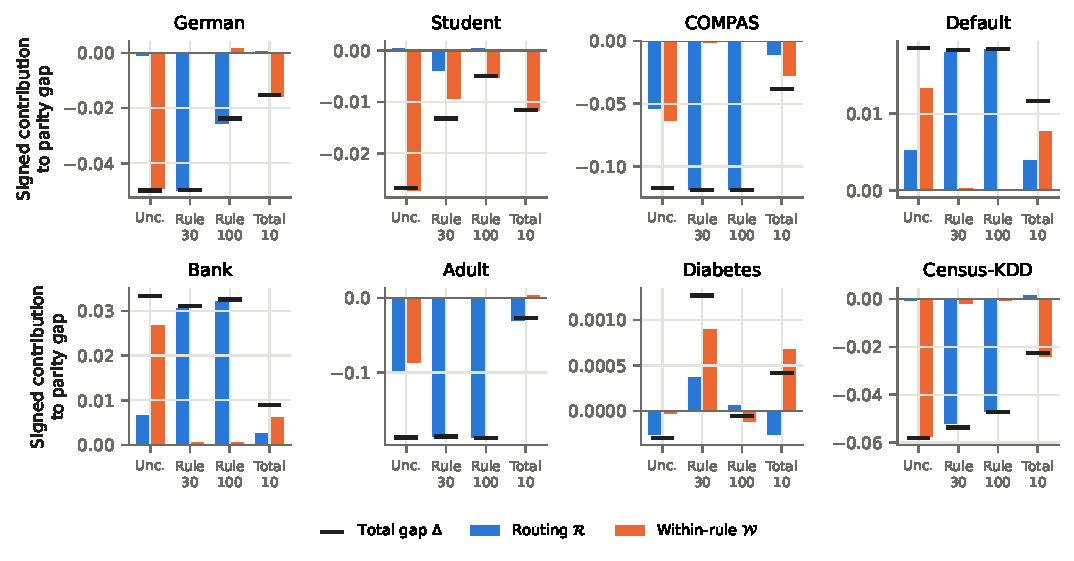
\includegraphics[width=1\textwidth,height=\textheight]{figures/fig_displacement.pdf}
\caption{Theorem 1 decomposition of the score-level gap (mean over splits) for the unconstrained model (Unc.), the rule-local penalty (Rule, λ = 30 and 100) and the total penalty (Total, λ = 10)}
\end{figure}

\emph{Where the gap sits.} On Adult and COMPAS both terms are substantial: the groups are routed to different rules \emph{and} treated differently within rules. On Census-KDD, German, Student and Bank the gap is almost entirely within-rule.

\emph{The rule-local penalty removes \(\mathcal W\) but not the gap} on the two datasets with a large gap. On Adult, \(\mathcal W\) falls to zero while \(\mathcal R\) grows from −0.101 to −0.188, and the decision-level FDP stays at 0.187--0.189 (score level: −0.187 and −0.188); on COMPAS it stays at 0.227--0.237. Accuracy is unchanged. The shift of \(\mathcal R\) (0.087 on Adult, 0.064 on COMPAS) is an order of magnitude larger than its bootstrap standard deviation over test resamples (0.002--0.005 and 0.002--0.011; Table S14). The total penalty shrinks both terms (Adult FDP 0.015). On the other datasets the evidence is weaker. On Bank and Default the gap is about 0.02 to begin with; on Census-KDD the penalty lowers it from 0.048 to 0.037, so displacement is partial; on German and Student it lowers FDP to 0.036 and 0.007, so displacement does not occur, although with test sets of 200 and 130 instances these results are noisy (the bootstrap standard deviation of the German gap is 0.019--0.028, and FDP at \(\lambda = 30\) is 0.072). Real data thus show complete displacement on two datasets, partial on one and none on two. With the fuzzy group \emph{young} on Adult the result is the same as for sex: the rule-local penalty (\(\lambda = 100\)) removes \(\mathcal W\) (−0.085 to 0.000) while \(\mathcal R\) grows from −0.116 to −0.201, so the score-level gap stays at −0.201 against −0.200 and the decision-level FDP at 0.189 against 0.191 (Nadeau--Bengio \(p = 0.79\); Table S19). The controlled test is in Section 6.4.

\emph{Displacement does not depend on the regularisers or on fuzzy antecedents.} With the plain protocol (log-loss and rule-local penalty only, no early stopping), the penalty again removes \(\mathcal W\) and leaves the gap in place (COMPAS FDP 0.211 without and 0.218 with it; Adult 0.183 and 0.177). A mixture of experts with a linear softmax gate instead of fuzzy antecedents \cite{jacobs}, with the same consequents and training, shows the same pattern (COMPAS 0.228 and 0.231, Adult 0.185 and 0.185; Table S17). Displacement is a property of models with learned routing and a locally constrained output, not of fuzzy systems; the fuzzy rule base contributes readable antecedents for the regions involved.

\emph{Displacement is not an artefact of the weighting or of a loss of fit.} With the coverage and rates of either group as Oaxaca--Blinder reference instead of midpoints, \(\mathcal W\) of the unconstrained model is −0.076 or −0.097 on Adult and −0.066 or −0.061 on COMPAS, and under the rule-local penalty it is 0.000 for all three weightings (Table S18). Test log-loss is 0.318, 0.316 and 0.318 for the first-order, rule-local and zero-order models on Adult and 0.601, 0.600 and 0.600 on COMPAS: the first-order consequents add no measurable fit, which is the case in which Theorem 2 predicts that the rule-local penalty leaves the gap in place. On COMPAS the penalty reduces the usage-weighted norm of the consequent slopes from 1.15 to 0.28, moving the model towards a zero-order rule base; on Adult the norm changes little (1.77 to 1.60) and \(\mathcal W\) vanishes nonetheless.

\hypertarget{a-controlled-test-of-theorem-2}{%
\subsection{A controlled test of Theorem 2}\label{a-controlled-test-of-theorem-2}}

Table 6 and Fig. 3 report the synthetic study for \(\rho = 0.6\). The retained gap is the ratio of the score-level gap after the penalty to the unconstrained gap.

\begin{longtable}[]{@{}
  >{\raggedright\arraybackslash}p{(\columnwidth - 16\tabcolsep) * \real{0.1111}}
  >{\raggedright\arraybackslash}p{(\columnwidth - 16\tabcolsep) * \real{0.1111}}
  >{\raggedright\arraybackslash}p{(\columnwidth - 16\tabcolsep) * \real{0.1111}}
  >{\raggedright\arraybackslash}p{(\columnwidth - 16\tabcolsep) * \real{0.1111}}
  >{\raggedright\arraybackslash}p{(\columnwidth - 16\tabcolsep) * \real{0.1111}}
  >{\raggedright\arraybackslash}p{(\columnwidth - 16\tabcolsep) * \real{0.1111}}
  >{\raggedright\arraybackslash}p{(\columnwidth - 16\tabcolsep) * \real{0.1111}}
  >{\raggedright\arraybackslash}p{(\columnwidth - 16\tabcolsep) * \real{0.1111}}
  >{\raggedright\arraybackslash}p{(\columnwidth - 16\tabcolsep) * \real{0.1111}}@{}}
\caption{Synthetic study (\(\rho = 0.6\), mean ± s.d. over 5 seeds). \(\hat\varepsilon_0\): excess risk of a zero-order rule base with the same \(L\) and antecedent mode (an upper bound on \(\varepsilon_\Omega\)); \(\Delta_0\): unconstrained score-level gap; retained gap = \(\Delta_\lambda/\Delta_0\). The total penalty was run for all \(L\) in the linear scenario and for \(L \in \{1,16\}\) in the nonlinear one.}\tabularnewline
\toprule\noalign{}
\begin{minipage}[b]{\linewidth}\raggedright
\textbf{Scenario}
\end{minipage} & \begin{minipage}[b]{\linewidth}\raggedright
\textbf{Antecedents}
\end{minipage} & \begin{minipage}[b]{\linewidth}\raggedright
\(L\)
\end{minipage} & \begin{minipage}[b]{\linewidth}\raggedright
\(\hat\varepsilon_0\) \textbf{(nats)}
\end{minipage} & \begin{minipage}[b]{\linewidth}\raggedright
\(\Delta_0\)
\end{minipage} & \begin{minipage}[b]{\linewidth}\raggedright
\textbf{Retained score gap, rule-local} \(\lambda=100\)
\end{minipage} & \begin{minipage}[b]{\linewidth}\raggedright
\textbf{Retained score gap, total} \(\lambda=100\)
\end{minipage} & \begin{minipage}[b]{\linewidth}\raggedright
\textbf{Retained decision gap, rule-local / total}
\end{minipage} & \begin{minipage}[b]{\linewidth}\raggedright
\(|\mathcal W|\) \textbf{after rule-local}
\end{minipage} \\
\midrule\noalign{}
\endfirsthead
\toprule\noalign{}
\begin{minipage}[b]{\linewidth}\raggedright
\textbf{Scenario}
\end{minipage} & \begin{minipage}[b]{\linewidth}\raggedright
\textbf{Antecedents}
\end{minipage} & \begin{minipage}[b]{\linewidth}\raggedright
\(L\)
\end{minipage} & \begin{minipage}[b]{\linewidth}\raggedright
\(\hat\varepsilon_0\) \textbf{(nats)}
\end{minipage} & \begin{minipage}[b]{\linewidth}\raggedright
\(\Delta_0\)
\end{minipage} & \begin{minipage}[b]{\linewidth}\raggedright
\textbf{Retained score gap, rule-local} \(\lambda=100\)
\end{minipage} & \begin{minipage}[b]{\linewidth}\raggedright
\textbf{Retained score gap, total} \(\lambda=100\)
\end{minipage} & \begin{minipage}[b]{\linewidth}\raggedright
\textbf{Retained decision gap, rule-local / total}
\end{minipage} & \begin{minipage}[b]{\linewidth}\raggedright
\(|\mathcal W|\) \textbf{after rule-local}
\end{minipage} \\
\midrule\noalign{}
\endhead
\bottomrule\noalign{}
\endlastfoot
linear & trainable & 1 & 0.2353 & −0.216 & 0.01 ±~0.01 & 0.01 ±~0.01 & 0.02 / 0.02 & 0.0024 \\
linear & trainable & 2 & 0.0006 & −0.219 & 1.01 ±~0.01 & 0.00 ±~0.02 & 1.01 / 0.08 & 0.0000 \\
linear & trainable & 4 & 0.0010 & −0.218 & 1.01 ±~0.01 & 0.01 ±~0.02 & 1.01 / 0.13 & 0.0000 \\
linear & trainable & 8 & 0.0013 & −0.216 & 1.01 ±~0.02 & 0.01 ±~0.01 & 1.00 / 0.12 & 0.0000 \\
linear & trainable & 16 & 0.0013 & −0.215 & 1.01 ±~0.02 & 0.01 ±~0.01 & 1.01 / 0.10 & 0.0000 \\
linear & trainable & 32 & 0.0019 & −0.217 & 0.99 ±~0.01 & 0.00 ±~0.02 & 1.00 / 0.08 & 0.0001 \\
linear & fixed & 4 & 0.1576 & −0.215 & 0.22 ±~0.06 & --- & 0.37 / --- & 0.0035 \\
linear & fixed & 16 & 0.1336 & −0.214 & 0.31 ±~0.07 & --- & 0.52 / --- & 0.0031 \\
nonlinear & trainable & 1 & 0.2832 & −0.192 & 0.01 ±~0.00 & 0.01 ±~0.00 & 0.01 / 0.01 & 0.0027 \\
nonlinear & trainable & 2 & 0.1723 & −0.192 & 0.59 ±~0.24 & --- & 0.77 / --- & 0.0032 \\
nonlinear & trainable & 4 & 0.0276 & −0.194 & 0.99 ±~0.03 & --- & 1.03 / --- & 0.0006 \\
nonlinear & trainable & 8 & 0.0066 & −0.193 & 1.01 ±~0.01 & --- & 1.01 / --- & 0.0001 \\
nonlinear & trainable & 16 & 0.0051 & −0.195 & 1.00 ±~0.01 & 0.00 ±~0.01 & 1.00 / 0.16 & 0.0001 \\
nonlinear & trainable & 32 & 0.0048 & −0.195 & 1.00 ±~0.01 & --- & 1.01 / --- & 0.0000 \\
nonlinear & fixed & 4 & 0.2401 & −0.169 & 0.37 ±~0.15 & --- & 0.53 / --- & 0.0027 \\
nonlinear & fixed & 16 & 0.2231 & −0.166 & 0.51 ±~0.11 & --- & 0.73 / --- & 0.0017 \\
\end{longtable}

\begin{figure}
\centering
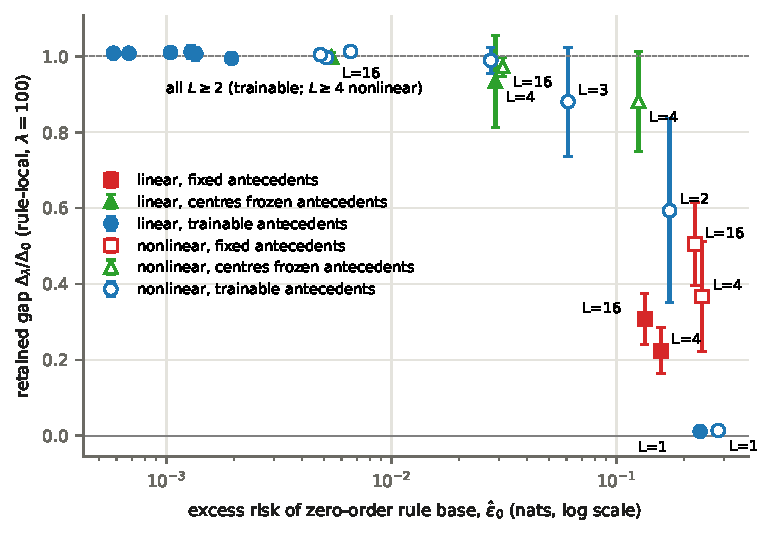
\includegraphics[width=1\textwidth,height=\textheight]{figures/fig_synth_displacement.pdf}
\caption{Share of the gap retained under the rule-local penalty (λ = 100) against the excess risk of a zero-order rule base with the same antecedent family (log scale), for both scenarios and for trainable, centres-frozen (Table S21) and fixed antecedents (ρ = 0.6, mean ± s.d. over 5 seeds)}
\end{figure}

\begin{itemize}
\tightlist
\item
  \emph{Complete displacement when \(\hat\varepsilon_0\) is small.} With trainable antecedents and \(L \geq 2\) (linear) or \(L \geq 4\) (nonlinear), \(\hat\varepsilon_0 \leq 0.028\) nats and the rule-local penalty retains 0.99--1.01 of the gap while \(|\mathcal W| \leq 0.0006\); the total penalty removes it (retained ≤ 0.01). The result is the same for \(\rho = 0.3\) and \(0.9\).
\item
  \emph{No displacement with one rule.} For \(L = 1\) the rule-local penalty retains 0.01 of the gap, like the total penalty (Corollary 2).
\item
  \emph{Partial displacement when routing is restricted.} With frozen antecedents (\(\hat\varepsilon_0\) = 0.13--0.24) the penalty retains 0.22--0.51 of the gap, and in the nonlinear scenario with \(L = 2\) (\(\hat\varepsilon_0 = 0.17\)) 0.59 ± 0.24. The same penalty removes half to three quarters of the gap when the antecedents cannot move and none of it when they can, which shows directly that the gap is re-routed.
\end{itemize}

Further configurations fill the range of \(\hat\varepsilon_0\) between 0.028 and 0.13 nats (Table S21). With trainable antecedents and \(L = 3\) in the nonlinear scenario (\(\hat\varepsilon_0 = 0.061\)) and with frozen centres but trainable widths and gates (\(\hat\varepsilon_0 = 0.005\)--0.125), the penalty retains 0.88--1.00 of the gap, at a cost of up to five accuracy points; with centres, widths and gates frozen, \(\hat\varepsilon_0\) stays at 0.13 (linear) and 0.22 (nonlinear) up to \(L = 128\), and the retained gap at 0.32--0.54. Near \(\hat\varepsilon_0 = 0.13\) the retained gap is 0.88 in one configuration and 0.32 in another. \(\hat\varepsilon_0\) is thus an upper bound that guarantees displacement when it is small, not a predictor of the retained share when it is not; what separates the cases is whether the memberships can move, and trainable widths and gates suffice. We do not claim a threshold. At decision level the retained gap is 0.99--1.02 in the configurations with complete displacement. The bound of Corollary 3 held in all 80 alignment runs under both protocols, with the observed deviation at most 0.21 of it; the regulariser and optimisation-gap terms that separate Corollary 3 from Theorem 2 were at most 0.018 and between −0.061 and +0.015 nats, and displacement was the same under both protocols (Table S20).

\hypertarget{a-rule-level-audit-and-proxy-removal}{%
\subsection{A rule-level audit and proxy removal}\label{a-rule-level-audit-and-proxy-removal}}

Table 7 shows the rules with the largest shares (Section 4.2) of the gap of a zero-order FairTSK on Adult (split 0), without a penalty and with \(\lambda_f = 10\). For a zero-order rule base the gap is pure routing (Corollary 1). The table describes one model and is an illustration, not evidence about Adult; Table 8 then repeats the experiment without the marital variables over 10 splits.

\begin{longtable}[]{@{}
  >{\raggedright\arraybackslash}p{(\columnwidth - 10\tabcolsep) * \real{0.1667}}
  >{\raggedright\arraybackslash}p{(\columnwidth - 10\tabcolsep) * \real{0.1667}}
  >{\raggedright\arraybackslash}p{(\columnwidth - 10\tabcolsep) * \real{0.1667}}
  >{\raggedright\arraybackslash}p{(\columnwidth - 10\tabcolsep) * \real{0.1667}}
  >{\raggedright\arraybackslash}p{(\columnwidth - 10\tabcolsep) * \real{0.1667}}
  >{\raggedright\arraybackslash}p{(\columnwidth - 10\tabcolsep) * \real{0.1667}}@{}}
\caption{Rules with the largest centred share of the gap, zero-order FairTSK on Adult (split 0). Antecedents: the six with the largest relevance \(\varrho_{lj}\), centres in original units (``\textless{}'', ``\textgreater{}'': centre outside the observed range; ``(absent)'': the rule prefers the category to be absent). The share of rule \(l\) is \((m_{l}^{G} - m_{l}^{\neg G})(g_{l} - c)\), with \(c\) the mean score.}\tabularnewline
\toprule\noalign{}
\begin{minipage}[b]{\linewidth}\raggedright
\textbf{λ}
\end{minipage} & \begin{minipage}[b]{\linewidth}\raggedright
\textbf{Rule}
\end{minipage} & \begin{minipage}[b]{\linewidth}\raggedright
\textbf{Antecedents (six most relevant)}
\end{minipage} & \begin{minipage}[b]{\linewidth}\raggedright
\(g_l\)
\end{minipage} & \begin{minipage}[b]{\linewidth}\raggedright
\textbf{Coverage women / men}
\end{minipage} & \begin{minipage}[b]{\linewidth}\raggedright
\textbf{Centred share}
\end{minipage} \\
\midrule\noalign{}
\endfirsthead
\toprule\noalign{}
\begin{minipage}[b]{\linewidth}\raggedright
\textbf{λ}
\end{minipage} & \begin{minipage}[b]{\linewidth}\raggedright
\textbf{Rule}
\end{minipage} & \begin{minipage}[b]{\linewidth}\raggedright
\textbf{Antecedents (six most relevant)}
\end{minipage} & \begin{minipage}[b]{\linewidth}\raggedright
\(g_l\)
\end{minipage} & \begin{minipage}[b]{\linewidth}\raggedright
\textbf{Coverage women / men}
\end{minipage} & \begin{minipage}[b]{\linewidth}\raggedright
\textbf{Centred share}
\end{minipage} \\
\midrule\noalign{}
\endhead
\bottomrule\noalign{}
\endlastfoot
0 & R9 & age High (≈51.6) ∧ education-num High (≈15.4) ∧ marital-status = married ∧ hours-per-week High (≈69.7) ∧ occupation = other-service (absent) ∧ relationship = unmarried (absent) & 0.99 & 0.018 / 0.074 & −0.042 \\
0 & R6 & education-num High (\textgreater16) ∧ age High (≈53.7) ∧ relationship = own-child (absent) ∧ hours-per-week High (≈55.3) ∧ occupation = other-service (absent) ∧ marital-status = never-married (absent) & 0.98 & 0.016 / 0.065 & −0.036 \\
0 & R12 & education-num Low (≈4.47) ∧ capital-gain Low (\textless0) ∧ capital-loss Low (\textless0) ∧ marital-status = married (absent) ∧ fnlwgt Low (\textless1.38e+04) ∧ hours-per-week Low (≈21.3) & 0.01 & 0.154 / 0.059 & −0.023 \\
0 & R7 & capital-gain Low (\textless0) ∧ marital-status = married (absent) ∧ education-num Low (≈4.44) ∧ hours-per-week Low (≈12.4) ∧ occupation = exec-managerial (absent) ∧ relationship = husband (absent) & 0.01 & 0.136 / 0.066 & −0.016 \\
0 & R2 & hours-per-week Low (≈5.47) ∧ capital-gain Low (\textless0) ∧ education-num Low (≈5.37) ∧ marital-status = married (absent) ∧ occupation = prof-specialty (absent) ∧ capital-loss Low (\textless0) & 0.00 & 0.107 / 0.043 & −0.016 \\
0 & Σ all 16 rules & & & & −0.1953 (direct: −0.1953) \\
10 & R14 & age High (≈71.2) ∧ education-num High (\textgreater16) ∧ marital-status = married ∧ marital-status = never-married (absent) ∧ relationship = not-in-family (absent) ∧ relationship = wife & 0.95 & 0.094 / 0.032 & +0.044 \\
10 & R6 & relationship = own-child (absent) ∧ education-num High (\textgreater16) ∧ age High (≈54.6) ∧ hours-per-week High (≈58.1) ∧ occupation = handlers-cleaners (absent) ∧ marital-status = never-married (absent) & 0.95 & 0.022 / 0.067 & −0.032 \\
10 & R9 & age High (≈63.7) ∧ hours-per-week High (≈68.4) ∧ education-num High (\textgreater16) ∧ relationship = not-in-family (absent) ∧ marital-status = never-married (absent) ∧ occupation = other-service (absent) & 0.90 & 0.022 / 0.066 & −0.029 \\
10 & R15 & age Low (\textless17) ∧ capital-gain Low (\textless0) ∧ capital-loss Low (\textless0) ∧ hours-per-week Low (≈15.6) ∧ occupation = prof-specialty (absent) ∧ marital-status = never-married & 0.01 & 0.134 / 0.065 & −0.016 \\
10 & R10 & age High (≈80.1) ∧ capital-gain Low (\textless0) ∧ capital-loss Low (\textless0) ∧ relationship = own-child (absent) ∧ relationship = husband ∧ marital-status = never-married (absent) & 0.03 & 0.048 / 0.093 & +0.009 \\
10 & Σ all 16 rules & & & & −0.0306 (direct: −0.0306) \\
\end{longtable}

Without a penalty the gap (−0.195) has two sources: two high-score rules combining high age, education and hours with \emph{married} status cover men about four times as heavily as women, and three low-score rules combining low education and few hours with the \emph{absence} of married status cover women 2.1--2.6 times as heavily as men. With the penalty the gap shrinks to −0.031, partly through a high-score rule whose antecedents include \emph{married} and \emph{relationship = wife} and which covers women three times as heavily as men (+0.044): the penalty reduced the gap by targeting a subgroup of women through a proxy. The rules are readable but imperfect as linguistic statements. Labels such as \emph{High} and \emph{Low} are attached to learned Gaussian centres, not to a fixed linguistic partition; some centres lie outside the observed range; and some antecedents are redundant (e.g.~\emph{married} together with \emph{never-married (absent)}).

\begin{longtable}[]{@{}
  >{\raggedright\arraybackslash}p{(\columnwidth - 12\tabcolsep) * \real{0.1429}}
  >{\raggedright\arraybackslash}p{(\columnwidth - 12\tabcolsep) * \real{0.1429}}
  >{\raggedright\arraybackslash}p{(\columnwidth - 12\tabcolsep) * \real{0.1429}}
  >{\raggedright\arraybackslash}p{(\columnwidth - 12\tabcolsep) * \real{0.1429}}
  >{\raggedright\arraybackslash}p{(\columnwidth - 12\tabcolsep) * \real{0.1429}}
  >{\raggedright\arraybackslash}p{(\columnwidth - 12\tabcolsep) * \real{0.1429}}
  >{\raggedright\arraybackslash}p{(\columnwidth - 12\tabcolsep) * \real{0.1429}}@{}}
\caption{Adult with and without marital status and relationship (first-order FairTSK, test data, means over 10 splits, all s.d. below 0.01). Last columns: AUC for sex of the normalised firing of the four rules with the largest absolute share versus the other twelve, and single-feature AUC for sex of the three most relevant features of those four rules versus all features.}\tabularnewline
\toprule\noalign{}
\begin{minipage}[b]{\linewidth}\raggedright
\textbf{Inputs}
\end{minipage} & \begin{minipage}[b]{\linewidth}\raggedright
\textbf{Model}
\end{minipage} & \begin{minipage}[b]{\linewidth}\raggedright
\textbf{Accuracy}
\end{minipage} & \begin{minipage}[b]{\linewidth}\raggedright
\textbf{FDP}
\end{minipage} & \begin{minipage}[b]{\linewidth}\raggedright
\(\mathcal R\) / \(\mathcal W\)
\end{minipage} & \begin{minipage}[b]{\linewidth}\raggedright
\textbf{Sex AUC of firing: top-4 / other rules}
\end{minipage} & \begin{minipage}[b]{\linewidth}\raggedright
\textbf{Sex AUC of features: top-4 rules / all}
\end{minipage} \\
\midrule\noalign{}
\endfirsthead
\toprule\noalign{}
\begin{minipage}[b]{\linewidth}\raggedright
\textbf{Inputs}
\end{minipage} & \begin{minipage}[b]{\linewidth}\raggedright
\textbf{Model}
\end{minipage} & \begin{minipage}[b]{\linewidth}\raggedright
\textbf{Accuracy}
\end{minipage} & \begin{minipage}[b]{\linewidth}\raggedright
\textbf{FDP}
\end{minipage} & \begin{minipage}[b]{\linewidth}\raggedright
\(\mathcal R\) / \(\mathcal W\)
\end{minipage} & \begin{minipage}[b]{\linewidth}\raggedright
\textbf{Sex AUC of firing: top-4 / other rules}
\end{minipage} & \begin{minipage}[b]{\linewidth}\raggedright
\textbf{Sex AUC of features: top-4 rules / all}
\end{minipage} \\
\midrule\noalign{}
\endhead
\bottomrule\noalign{}
\endlastfoot
all features & unconstrained & 0.852 & 0.189 & −0.101 / −0.086 & 0.628 / 0.605 & 0.590 / 0.522 \\
all features & rule-local, λ=100 & 0.853 & 0.187 & −0.188 / 0.000 & 0.693 / 0.688 & 0.601 / 0.522 \\
without marital, relationship & unconstrained & 0.825 & 0.108 & −0.056 / −0.052 & 0.585 / 0.554 & 0.552 / 0.512 \\
without marital, relationship & rule-local, λ=100 & 0.826 & 0.102 & −0.108 / 0.000 & 0.612 / 0.575 & 0.557 / 0.512 \\
without marital, relationship & total, λ=10 & 0.818 & 0.058 & −0.027 / −0.003 & --- & --- \\
without marital, relationship & total, λ=100 & 0.811 & 0.045 & −0.011 / +0.005 & --- & --- \\
\end{longtable}

Removing the two variables roughly halves the unconstrained gap (0.189 to 0.108) at a cost of 2.7 accuracy points, but displacement persists: under the rule-local penalty the gap is 0.102, with \(\mathcal W = 0\) (the small reduction is not significant: Nadeau--Bengio \(p = 0.08\)). Only the total penalty closes the gap (0.058 at \(\lambda = 10\)). Without the marital variables, the firing of the four rules carrying the gap is slightly more associated with sex than that of the other rules (AUC 0.612 versus 0.575, Nadeau--Bengio \(p = 0.003\)), and their most relevant features are slightly more associated with sex than the average feature (0.557 versus 0.512, \(p < 0.001\)), led by hours per week (single-feature AUC 0.65). These are small effects. The same features would be found by a feature-level attribution of the gap \cite{begley}. What the decomposition adds is the information that the gap now runs \emph{between} rules rather than within them, which is exactly what a within-rule audit would miss.

\hypertarget{discussion-and-limitations}{%
\section{Discussion and limitations}\label{discussion-and-limitations}}

\textbf{What the fuzzy rule base contributes.} The experiments separate two claims that are often made together for neuro-fuzzy models. The first, that a fuzzy rule base yields a better accuracy--fairness trade-off, is not supported: FairTSK and a ReLU network with the same penalty cannot be distinguished. The second, that it makes a model's unfairness legible, holds in a limited sense. The decomposition shows where a gap sits, and it exposes a behaviour, displacement, that every scalar metric of Section 6.1 misses. But the decomposition applies to any convex mixture, including mixtures of experts and decision trees; displacement occurs in a mixture of experts without fuzzy antecedents; and fair trees and rule lists are much shorter and match FairTSK's front on several datasets. What the fuzzy formulation adds is specific: a protected group stated as a linguistic term with an explicit membership function, and soft, linguistically labelled regions to which a routing share can be attributed.

\textbf{Implications.} (i) Local and group criteria must be stated and audited separately: requiring that individuals who match the same rule be treated alike leaves the group gap within \(\kappa_\mu\sqrt{\varepsilon_\Omega/(2\pi(1-\pi))}\) of the Bayes gap, and on Adult and COMPAS it left it within 0.01 of the unconstrained model. This is a concrete case of the concern that conditional parity with respect to learned strata can be satisfied while the group disparity persists \cite{lipton,kearns}. (ii) More flexible routing displaces more; restricting it (a single rule, fixed antecedents) restores the effect of a local penalty, at the price of accuracy. (iii) Removing proxies is not a remedy if the remaining features still let the antecedents separate the groups. (iv) A penalty for a named group is itself local along the axis of the sensitive variable: FDP for \emph{young} moved disparity to the over-60s on Bank. The specification of the protected group is therefore a normative decision that the penalty cannot make, and the bands it leaves out need to be audited too.

\textbf{Limitations.}

\begin{itemize}
\tightlist
\item
  \emph{Theory.} Theorem 2 is a sufficient, population-level condition whose constant is not tight; \(\varepsilon_\Omega\), and hence the certificate of Corollary 3, requires \(\eta\) and is available only on synthetic data. We give no necessary conditions and no finite-sample bounds; the mini-batch estimates of (5) are ratios and can be noisy for rules that cover few members of a group. The Lipschitz bound of Proposition S1 is not informative in practice.
\item
  \emph{Decomposition.} The split into \(\mathcal R\) and \(\mathcal W\) and the rule shares depend on the parametrisation; they explain the fitted model, not the data. Theorem 1 concerns scores, not decisions. Rule-level attributions are not stable across splits or after compaction; only the features that carry the gap are (Table S23; Table S22).
\item
  \emph{Interpretability.} First-order consequents are dense (on average 8 to 386 non-zero weights per rule, depending on the dataset); every rule fires everywhere to some degree; antecedent labels are attached to learned centres; no human-subject evaluation was carried out. We did not compare the audit empirically with Shapley-based attributions of the gap \cite{begley}, which answer a different question (which features, not which model components).
\item
  \emph{Experiments.} Displacement on real data is complete on two datasets, partial on one and absent on two small, noisy ones. Six of the eight main groups are crisp; the fuzzy group was tested on German and Bank and, in a separate run, on Adult. Baselines were run on small fixed grids rather than tuned to a common budget; HV favours families with more configurations; only demographic parity was enforced, which raised equalised-odds differences and made the COMPAS operating points nearly trivial. Hyperparameters of FairTSK were fixed in a pilot on split 0 of two datasets; removing that split changed no conclusion. Adult reflects 1994 census data \cite{ding}, and COMPAS labels encode policing practices \cite{compas}.
\end{itemize}

\hypertarget{conclusion}{%
\section{Conclusion}\label{conclusion}}

Fuzzy set theory was used for two purposes: to define protected groups by membership functions (fuzzy demographic parity) and to decompose a group gap inside a TSK classifier into routing and within-rule parts. The decomposition shows that a rule-local penalty, a learned form of conditional statistical parity, can remove within-rule disparity while the group gap survives through re-routing. We gave a sufficient condition for this displacement, extended it to regularised and approximately trained models, confirmed it where the Bayes score is known, and observed it on Adult and COMPAS and in a mixture of experts without fuzzy antecedents. The fairness-aware TSK classifier is as good as, not better than, a neural network with the same penalty. The practical lesson is that local fairness constraints and group parity must be audited separately, and that a fuzzy group specification makes explicit, but does not settle, whom a parity constraint protects. Extending the decomposition to error-rate criteria and intersecting fuzzy groups, and deriving necessary conditions for displacement, are open problems.

\hypertarget{statements-and-declarations}{%
\section{Statements and Declarations}\label{statements-and-declarations}}

\textbf{Funding.} This research did not receive any specific grant from funding agencies in the public, commercial, or not-for-profit sectors.

\textbf{Competing interests.} The author has no relevant financial or non-financial interests to disclose.

\textbf{Ethics approval and consent.} Not applicable: the study uses only publicly available, de-identified benchmark datasets.

\textbf{Author contributions.} R. Imamguluyev: conceptualization, methodology, formal analysis, software, investigation, validation, data curation, visualization, writing -- original draft, writing -- review and editing.

\textbf{Data availability.} All datasets are publicly available: Adult, Statlog (German Credit), Bank Marketing, Default of Credit Card Clients, Student Performance, Diabetes 130-US Hospitals and Census-Income (KDD) from the UCI Machine Learning Repository, and COMPAS from the ProPublica repository \cite{compas}.

\textbf{Code availability.} The model and preprocessing code, per-split results, the synthetic-study code and the scripts that generate every table and figure are archived on Zenodo \cite{software} (https://doi.org/{[}ZENODO-v1.1-DOI{]}) and developed at https://github.com/rahibaydinoglu-byte/fuzzy-demographic-parity; in the code, FairTSK is called ZadehNet.

\textbf{Use of generative AI.} The use of a large language model is described in Section 5 (Implementation and use of AI tools).
